\chapter{O ciclo de vida do produto na I4.0}
\label{cha:ciclo-de-vida}
	
	Este capítulo visa trazer discussões sobre o impacto do amplo compartilhamento da memória digital do produto ao longo da cadeia de suprimentos por meio serviços na Indústria 4.0.
	
	São abordadas possíveis mudanças na curva de ciclo de vida do produto e o surgimento de novos modelos de negócio baseado em dados (\textit{data-driven}).
	
	Uma visão da MDP sobre o eixo ``Ciclo de Vida e Cadeia de Valor'' do RAMI4.0 é abordada, discutindo melhor o porquê e as atribuições dos AASs como ``tipos'' e como ``instâncias''.
	

\section{Ciclo de vida do produto no RAMI4.0}

	O modelo do RAMI4.0 apresenta um eixo de ciclo de vida generalizado, derivado da norma IEC 62890 \cite{adolphs2015rami}. A ideia do trás do eixo Ciclo de Vida e Cadeia de Valor é representar, como o nome diz, o ciclo de vida de um Componente I4.0 ao longo de toda a sua cadeia de valor.
	
	Os tipos estão presentes desde a concepção/conceitualização até os primeiros protótipos/testes. O tipo de um ativo é definido pelas suas propriedades e funcionalidades distintas. Todos os itens que são criados ao longo do projeto de um produto (e.g., desenhos em CAD, manuais, \textit{softwares}, etc) são incorporados ao tipo do ativo. Informações externas associadas ao ativo que são criadas ao longo de seu desenvolvimento como informações de \textit{marketing} também são incorporadas ao tipo.
	
	As instâncias são criadas/produzidas com base nas informações de um tipo de ativo. Informações específicas sobre produção, logística, qualidade e testes são associadas à instância de um ativo. Na fase de instância do ativo, os dados de uso são coletados e associados para então poderem ser armazenados na MDP e compartilhados com outros parceiros ao longo da cadeia de suprimentos. 
	
	O histórico completo do ciclo de vida do produto está associados à combinação entre o tipo e a instância de um determinado produto. Estes dados podem ser aproveitados de forma inteligente para a geração de valor, gerando assim novos modelos de negócio.
	
	Os relacionamentos entre tipos e instâncias são cíclicos e possibilitam a retroalimentação de informações. Para os ativos de um produto, por exemplo, informações sobre seu uso e manutenção armazenadas na MDP podem auxiliar em melhorias no seu próprio processo de fabricação, além de ser fonte de dados para o desenvolvimento de novas versões aperfeiçoadas do mesmo produto, gerando um novo tipo.
	
	Portanto, o fluxo de informações entre tipos e instâncias de um produto são essenciais para a melhoria do projeto do produto. A \autoref{fig:aas-lifecycle} ilustra como ocorre a instancialização (criação de uma instância a partir de um tipo) e o uso da MDP das instâncias para a criação de novas versões de um tipo.
	
	\begin{figure}[htb!]
		\centering
		\caption{Ciclo de vida do produto.}
		\label{fig:aas-lifecycle}
		\includegraphics[width=0.9\textwidth]{aas-lifecycle}
		\fonte{O autor.}
	\end{figure}

\section{ Modelos de negócio orientados por dados }



\subsection{ Desenvolvimento do produto orientado por dados   }

\lipsum[1-1]

\subsection{ Manutenção do produto orientada por dados }

\lipsum[1-1]